%% ==============================
\chapter{Methoden der Dimensionsreduktion}
\label{ch:MethodenDerDimRed}
%% ==============================

Wie bereits in der Einleitung erwähnt wurde, haben kürzlich vor allem verschiedenste Varianten von
neuronalen Netzen einen hohen Grad an Aufmerksamkeit durch bemerkenswerte Errungenschaften auf
Gebieten der automatischen Spracherkennung oder \textit{Computer Vision} erlangt. Fraglich ist, ob
diese neuen Algorithmen auch auf dem Bereich der Dimensionsreduktion einen entscheidenden
Fortschritt gemacht haben. Deshalb wird von der üblichen Unterteilung (siehe
\secref{ch:Dimensionsreduktion:Ansaetze}) der Methoden abgewichen. Stattdessen werden die Methoden
in dieser Arbeit in statistische Methoden und Machine Learning Ansätze unterteilt, um diese
anschließend in \chapref{ch:Vergleich} gegenüberstellen zu können. Nachdem also die Motivation und
Idee in \chapref{ch:Enleitung}, sowie die Terminologie und mathematische Fundierung für die
Dimensionsreduktion in \chapref{ch:Dimensionsreduktion} besprochen wurde, werden nun zuerst die
statistischen Methoden in \secref{ch:MethodenDerDimRed:statistisch} und danach die Machine Learning
Ansätze in \secref{ch:MethodenDerDimRed:modern} erläutert.

\section{Statistische Methoden}
\label{ch:MethodenDerDimRed:statistisch}

Zu den statistischen Methoden, die in dieser Arbeit vorgestellt werden, gehören die
\newterm{Principal Component Analysis} (PCA) in \subsecref{ch:MethodenDerDimRed:statistisch:PCA}
und die nichtlineare Erweiterung \newterm{Kernel Principal Component Analysis} (Kernel PCA)
(\subsecref{ch:MethodenDerDimRed:statistisch:kPCA}). Außerdem wird \newterm{Locally Linear
	Embedding} (LLE) in \subsecref{ch:MethodenDerDimRed:statistisch:LLE} als Vertreter der
statistischen Methoden genauer behandelt.

%% ==============================
\subsection{Principal Component Analysis}
\label{ch:MethodenDerDimRed:statistisch:PCA}
\nomenclature[Z]{PCA}{Principal Component Analysis}

Die Principal Component Analysis ist \textit{die} Methode der Dimensionsreduktion und wurde
erstmals von \textcite{Pearson.1901} und \textcite{Hotelling.1933} entwickelt. Trotz des
mittlerweile relativ hohen Alters ist die Principal Component Analysis immer noch aufgrund der
simplen Anwendbarkeit oft eine erste Wahl für die Dimensionsreduktion. Im Folgenden wird auf die
zentrale Idee und Motivation der Principal Component Analysis, sowie die mathematische Herleitung
der sogenannten \newterm{Hauptkomponenten} (engl. \textit{principal components}) eingegangen.

\subsubsection{Grundidee}
\label{ch:MethodenDerDimRed:statistisch:PCA:Grundidee}
Die zentrale Idee der Principal Component Analysis ist die Transformation des Koordinatensystems in einer möglichst \textit{verlustfreien} Art und Weise. Verlustfrei bedeutet im Kontext der Principal Component Analysis, dass möglichst viel Variation in den Daten erhalten bleiben soll \parencite[vgl.][1]{Jolliffe.2002}. Das Ziel ist es also, die Richtungen der größten Varianz in den
Daten zu finden, da diese den höchsten Informationsgehalt besitzen. Daher wird sukzessive die
Varianz der im Folgenden definierten Hauptkomponenten maximiert. Dies führt dazu, dass die erste
Hauptkomponente die Richtung der größten Varianz abbildet, die zweite Hauptkomponente die Richtung
der zweitgrößten Varianz und so weiter, d.h. die weiteren Hauptkomponenten bilden sukzessive
weniger Varianz der ursprünglichen Variablen ab. Um nun die Dimension von $D$ auf $d$ zu
reduzieren, werden die Richtungen der größten Varianz, d.h. die ersten $d$ Hauptkomponenten
ausgewählt. Die Definition und Herleitung dieser Hauptkomponenten wird im nachfolgenden
Unterabschnitt genauer betrachtet.

\subsubsection{Herleitung der Hauptkomponenten}
\label{ch:MethodenDerDimRed:statistisch:PCA:HerleitungPC}

Als Ausgangsbasis wird ein $D$-dimensionaler Zufallsvektor $\rvect{x} = \tr{(\rv{x}_1, \ldots,
		\rv{x}_D)}$ mit $\Exp[\rvect{x}] = \vect{0}$ angenommen und das Ziel ist es, eine $d$-dimensionale
Repräsentation $\rvect{y} = \tr{(\rv{y_1},\ldots,\rv{y}_d)}$ zu erhalten. Daher wird $\rvect{y}$
nun als eine Linearkombination des ursprünglichen Vektors $\rvect{x}$ wie folgt ausgedrückt:
\begin{equation}
	\rv{y}_i = \tr{\vect{a}_i} \rvect{x} = a_{i1} \rv{x}_1 + \cdots + a_{iD} \rv{x}_D
	\quad \text{mit } i = 1,\ldots,d \,
\end{equation}
wobei $\vect{a}_i$ die \newterm{Koeffizienten} (auch: Ladungen) der $i$-ten Hauptkomponente $y_i$ sind \parencite[vgl.][2]{Jolliffe.2002}.\footnote{Wie \textcite[6]{Jolliffe.2002} hervorhebt, sollte der
	Begriff \enquote{Hauptkomponente} für die transformierten Variablen $y_1, \ldots, y_d$ und nicht
	für die Koeffizienten $a_1, \ldots, a_d$ verwendet werden, um Verwirrung zu vermeiden.} Durch diese
$d$ Gleichungen erhalten wir die neuen transformierten Merkmale $y_1, \ldots, y_d$.

Betrachtet wird nun zunächst lediglich die \textit{erste} Hauptkomponente $\tr{\vect{a}_1}
	\rvect{x}$. Wie zu Beginn erwähnt, soll möglichst viel Variation von der ursprünglichen
Repräsentation $\rvect{x}$ erhalten bleiben. Daher wird die erste Hauptkomponente so gewählt, dass
die Varianz maximal wird:
\begin{equation}
	\label{eq:PCA-Optimierungsproblem}
	\max_{\vect{a}_1}\, \Var \left( \tr{\vect{a}_1} \rvect{x} \right) = \max_{\vect{a}_1} \tr{\vect{a}_1} \mat{\Sigma} \vect{a}_1
\end{equation}
wobei $\mat{\Sigma}$ die Kovarianzmatrix von $\rvect{x}$ ist. Dieses Maximierungsproblem ist jedoch nach oben unbeschränkt, weshalb man zusätzlich die Bedingung
\begin{equation}
	\label{eq:PCA-Normierung-Vektor}
	\norm{ \vect{a}_1 }^2 = \tr{\vect{a}_1} \vect{a}_1 = 1
\end{equation}
zum nun \textit{restringierten} Maximierungsproblem hinzufügt. Dieses Problem kann mithilfe des Lagrange-Ansatzes gelöst werden. Es stellt sich heraus, dass sich das Problem auf ein Eigenwertproblem reduziert, d.h. $\vect{a}_1$ muss ein Eigenvektor der Kovarianzmatrix $\mat{\Sigma}$ sein \parencite[vgl.][4 -- 6]{Jolliffe.2002}. Die $D \times D$-Matrix $\mat{\Sigma}$ hat jedoch $D$
Eigenvektoren. Um herauszufinden, welcher davon zur ersten Hauptkomponente gehört, betrachtet man
erneut die zu maximierende Zielfunktion in \eqref{eq:PCA-Optimierungsproblem} unter der Kenntnis,
dass $\vect{a}_1$ ein Eigenvektor von $\mat{\Sigma}$ ist. Man erhält somit
\begin{equation}
	\tr{\vect{a}_1} \mat{\Sigma} \vect{a}_1 = \tr{\vect{a}_1} \lambda_1 \vect{a}_1 = \lambda_1 \tr{\vect{a}_1} \vect{a}_1 = \lambda_1 \, ,
\end{equation}
wobei im ersten Schritt die Eigenvektor-Eigenschaft und im letzten Schritt die Normierung des Vektors (\eqref{eq:PCA-Normierung-Vektor}) ausgenutzt wurde \parencite[5]{Jolliffe.2002}. Die Zielfunktion entspricht also gerade dem Eigenwert $\lambda_1$ des
Vektors $\vect{a}_1$. Daher wissen wir wegen der Maximierung der Varianz der ersten
Hauptkomponente, dass $\vect{a}_1$ der Eigenvektor mit dem größten zugehörigen Eigenwert sein muss.

Um nun die zweite Hauptkomponente zu erhalten, wird wieder die Varianz unter der Nebenbedingung
$\norm{\vect{a}_2}^2 = 1$ maximiert. Zusätzlich muss jedoch gelten, dass die zweite Hauptkomponente
zur Ersten unkorreliert ist \parencite[5]{Jolliffe.2002}, das heißt
\begin{equation}
	\label{eq:PCA-unkorreliertheit}
	\Cov(\tr{\vect{a}_1}\rvect{x}, \tr{\vect{a}_2}\rvect{x}) \overset{!}{=} 0 \, .
\end{equation}
Auch dieses Optimierungsproblem ist ein Eigenwertproblem und man erhält, dass die Koeffizienten $\vect{a}_2$ der zweiten Hauptkomponente der Eigenvektor mit dem zweitgrößten Eigenwert von $\mat{\Sigma}$ ist.\footnote{Die Bedingung, dass die zweite Hauptkomponente zur Ersten unkorreliert (orthogonal) sein muss, ist, wie sich durch simple Umformungen von \eqref{eq:PCA-unkorreliertheit} zeigen lässt, äquivalent zur Orthogonalität der beiden Vektoren $\vect{a}_1$ und $\vect{a}_2$. Da diese Vektoren Eigenvektoren sind und die Eigenvektoren jeder symmetrischen Matrix zwangsweise orthogonal sind, ändert diese Nebenbedingung das Ergebnis des Optimierungsproblems nicht.}
Generell lässt sich zeigen, dass die Koeffizienten der $i$-ten Hauptkomponente dem Eigenvektor mit dem $i$-ten nach der Größe geordneten Eigenwert entspricht \parencite[6]{Jolliffe.2002}. Aus diesem Grund lassen sich die Hauptkomponenten kompakt durch
\begin{equation}
	\rvect{y} = \tr{\mat{A}} \rvect{x}
\end{equation}
ausdrücken, wobei $\mat{A} = [\vect{a}_1,\ldots,\vect{a}_d] \in \real^{D \times d}$ die (Ladungs-)Matrix der Eigenvektoren als Spaltenvektoren ist und die Eigenvektoren nach absteigendem zugehörigen Eigenwert sortiert sind, d.h. $\lambda_1 > \lambda_2 > \cdots > \lambda_d$.

\subsubsection{Erweiterungen}
\label{ch:MethodenDerDimRed:statistisch:PCA:Erweiterungen}

Ein Schwachpunkt von PCA ist, dass die orthogonale Transformation auf die Eigenvektorbasis der
Kovarianzmatrix inhärent linear ist. Die Principal Component Analysis ist also in dieser
klassischen Form nicht in der Lage, eine nichtlineare Mannigfaltigkeit in den Daten zu erkennen.
Deswegen wurde unter anderem eine Generalisierung von PCA von \textcite{Scholkopf.1997} entwickelt,
die sogenannte \newterm{Kernel Principal Component Analysis} (Kernel PCA). Diese Methode wird in
\subsecref{ch:MethodenDerDimRed:statistisch:kPCA} genauer behandelt.

%% ==============================
\subsection{Kernel Principal Component Analysis}
\label{ch:MethodenDerDimRed:statistisch:kPCA}
\nomenclature[Z]{kPCA}{Kernel Principal Component Analysis}
Die Kernel Principal Components Analysis \parencite{Scholkopf.1997} ist eine nichtlineare Erweiterung der klassischen Principal Component
Analysis und kann somit theoretisch nichtlineare Zusammenhänge in den Daten erkennen. Um das zu
erreichen, wird der sogenannten \newterm{Kernel Trick} verwendet, der auch schon erfolgreich auf
\textit{Support Vector Machines} \parencite{Boser.1992} angewandt wurde. Im Folgenden wird die Grundidee der Kernel PCA und das Konzept
eines Kernels genauer erläutert. Daraufhin wird die konkrete Vorgehensweise vorgestellt und
abschließend werden praktische Probleme besprochen.

\subsubsection{Grundidee}
\label{ch:MethodenDerDimRed:statistisch:kPCA:Grundidee}

Die Grundidee der Kernel PCA ist es, die Daten mithilfe einer Funktion $\bm{\phi}$ in einen
Vektorraum $\mathcal{H}$ abzubilden, der nichtlinear mit dem Ursprungsraum $\mathcal{X}$ verbunden
ist. Der Raum $\mathcal{H}$ wird in diesem Kontext auch Merkmalsraum (engl. \textit{feature space})
genannt und kann potentiell sehr hochdimensional sein. Nach der Transformation wird die
traditionelle Principal Component Analysis durchgeführt, um damit die niedrigdimensionale
Repräsentation $\rvect{y}$ zu erhalten. Dieses Vorgehen erscheint auf den ersten Blick
kontraintuitiv, da durch den \enquote{Umweg} über die Abbildung $\bm{\phi}$ die Dimension zuerst
erhöht wird. Motiviert wird es dadurch, dass die Daten in $\mathcal{X}$ einen
\textit{nichtlinearen} Zusammenhang aufweisen können, während in $\mathcal{H}$ der Zusammenhang
linear und damit für lineare Algorithmen wie die Principal Component Analysis erkennbar ist \parencite[vgl.][26]{ShaweTaylor.2011}.

Der entscheidende Punkt ist, dass man die Abbildung $\bm{\phi}$ nicht explizit berechnet, sondern
mithilfe eines \newterm{Kernels} $\kappa: \mathcal{X} \times \mathcal{X} \rightarrow \real$
implizit gegeben hat \parencites[586 -- 588]{Bishop.2006}[583]{Scholkopf.1997}. Im Folgenden wird nach der Definition des
Kernels die Vorgehensweise der Kernel PCA genauer erläutert. Allerdings wird für eine eingehendere
Behandlung des Kernel Tricks und anderer Kernel-Methoden auf \textcite{ShaweTaylor.2011} verwiesen.

\subsubsection{Der Kernel}
\label{ch:MethodenDerDimRed:statistisch:kPCA:KernelFunktion}

Ein Kernel $\kappa$ ist definiert als das Skalarprodukt im Merkmalsraum \parencite[34]{ShaweTaylor.2011}
\begin{equation}
	\label{eq:kPCA:KernelFunction}
	\kappa(\vect{x}_i, \vect{x}_j) = \tr{\bm{\phi}(\vect{x}_i)} \bm{\phi}(\vect{x}_j)
\end{equation}
und ist damit intuitiv gesehen ein \enquote{Orakel} für die Ähnlichkeit der Daten im Merkmalsraum, weil dies ohne Kenntnis der Koordinaten berechnet werden kann \parencite[71]{ShaweTaylor.2011}. In der Praxis häufig anzutreffen sind Gaußsche Kernel (auch: Radiale
Basisfunktionen (RBF))
\begin{equation}
	\kappa(\vect{x}_i, \vect{x}_j) = \exp \left(- \frac{\norm{ \vect{x}_i - \vect{x}_j}^2}{2\sigma^2}\right) \, ,
\end{equation}
wobei der Parameter $\sigma > 0$ die Bandbreite des Kernels bestimmt \parencite[296]{ShaweTaylor.2011}. Ein zu großer Wert von $\sigma$ führt dazu, dass der Kernel fast
konstant wird und somit die lokale Struktur nicht mehr passend berücksichtigen kann. Ein zu kleiner
Wert führt zur Über- oder Unterschätzung der Ähnlichkeit zweier Punkte, d.h. der Kernel passt sich
zu sehr an die Daten an (Overfitting) \parencite[296 -- 297]{ShaweTaylor.2011}. Des Weiteren sind polynomiale Funktionen \parencite[292]{ShaweTaylor.2011}
\begin{equation}
	\kappa(\vect{x}_i, \vect{x}_j) = (\vect{x}_i \cdot \vect{x}_j)^p
\end{equation}
des Grades $p$ eine von vielen möglichen Kernel-Funktionen.

Der Kernel Trick besteht nun darin, den Algorithmus so umzuformen, dass $\bm{\phi}$ ausschließlich
als Skalarprodukt vorkommt. Diese Skalarprodukte können dann gemäß \eqref{eq:kPCA:KernelFunction}
durch die Kernel-Funktion ersetzt werden.

\subsubsection{Vorgehensweise}
\label{ch:MethodenDerDimRed:statistisch:kPCA:Vorgehensweise}

Betrachten wir also die Kovarianzmatrix $\mat{C}$ der in den Merkmalsraum projizierten Daten
$\bm{\phi}(\mat{X}) = \tr{\left[ \bm{\phi}(\vect{x}_1), \ldots, \bm{\phi}(\vect{x}_n) \right]}$. Um
die Berechnung zu vereinfachen, wird auch hier analog zur klassischen Principal Component Analysis
die Zentrierung der Daten im Merkmalsraum angenommen. Damit vereinfacht sich die Berechnung der
Kovarianzmatrix zu
\begin{equation}
	\mat{C} = \frac{1}{n} \tr{\bm{\phi}(\mat{X})} \bm{\phi}(\mat{X}) \, .
\end{equation}
Um nun die Principal Component Analysis durchführen zu können, müssten die Eigenvektoren dieser Matrix bestimmt werden. Dies ist jedoch nicht möglich, da die Abbildung $\bm{\phi}$ unbekannt ist. Wie sich herausstellt, ist diese Matrix aber ähnlich zur Kernel-Matrix $\mat{K}$, welche über den Kernel $\kappa$ als
\begin{align}
	\mat{K} & = \left( \kappa(\vect{x}_i, \vect{x}_j) \right)_{i,j = 1}^n \label{eq:kPCA:KernelMatrix_A} \\
	        & = \bm{\phi}(\mat{X}) \tr{\bm{\phi}(\mat{X})} \label{eq:kPCA:KernelMatrix_B}
\end{align}
definiert ist \parencites[68]{ShaweTaylor.2011}[584]{Scholkopf.1997}. Die Eigenwertzerlegung der zentrierten
Kernel-Matrix liefert mit einer entsprechenden Skalierung die Eigenvektoren der Kovarianzmatrix
$\mat{C}$. Konkret wird dazu die $n \times n$ Kernel-Matrix in einem ersten Schritt mittels
\begin{equation}
	\label{eq:KernelCentering}
	\widetilde{\mat{K}} = \mat{K} - \frac{1}{n} \ones \tr{\ones} \mat{K} - \frac{1}{n} \mat{K} \ones \tr{\ones} + \frac{1}{n^2} (\tr{\ones} \mat{K} \ones) \ones \tr{\ones}
\end{equation}
zentriert \parencite[131]{ShaweTaylor.2011}, wobei $\ones = \tr{(1, \ldots, 1)}$ der Vektor bestehend aus Einsen
ist. Diese Transformation der Kernel-Matrix stellt die Annahme der zentrierten Daten im
Merkmalsraum implizit sicher. Die zentrierte Kernel-Matrix $\widetilde{\mat{K}}$ wird dann im
zweiten Schritt in ihre Eigenvektoren $\vect{v_i}$ und Eigenwerte $\lambda_i$ mit $i = 1, \ldots,
	n$ zerlegt, womit über den Zusammenhang
\begin{equation}
	\label{eq:kPCA:ZusammenhangEigenvektoren}
	\vect{a}_i = \frac{1}{\sqrt{\lambda_i}} \vect{v}_i
\end{equation}
die Eigenvektoren $\vect{a}_i$ von $\mat{C}$ bestimmt werden können \parencite[142]{ShaweTaylor.2011}. Letztlich kann die Projektion eines Punktes $\vect{x}_i$ auf die
latente Repräsentation $\rvect{y}_i$ durch
\begin{equation}
	\vect{y}_i = \Bigg( \sum_{j=1}^n \vect{a}_j^{(l)} \kappa(\vect{x}_i, \vect{x}_j) \Bigg)_{l=1}^d
\end{equation}
berechnet werden, wobei $\vect{a}_j^{(l)}$ der $l$-te Eintrag in $\vect{a}_j$ ist \parencite[150]{ShaweTaylor.2011}.

\subsubsection{Praktische Probleme der Kernel PCA}
\label{ch:MethodenDerDimRed:statistisch:kPCA:AuswahlKF}

Ein entscheidender Schwachpunkt der Kernel PCA ist die Selektion der Hyperparameter, d.h. die
Auswahl des Kernels und die Wahl der Parameter für den Kernel. Problematisch ist ebenfalls, dass
der Kernel oft sensitiv gegenüber seiner Parameter ist. Im Falle eines Gaußschen Kernels muss ein
Parameter $\sigma$ gewählt werden, der die Bandbreite des Kernels bestimmt. Die Performance auf
einem Datensatz hängt davon ab, wie passend diese Bandbreite gewählt wurde. Allgemein umgeht man
das Problem der manuellen Auswahl eines Kernels und seiner Parameter für Kernel-Methoden mittels
einer Gittersuche und kombiniert dies mit Kreuzvalidierung \parencite[1]{Alam.2014}. Dabei wird ein Qualitätskriterium festgelegt und die Methode mit einer vorab
definierten Auswahl an Werten der Hyperparameter auf einer Teilmenge des Datensatzes trainiert und
mit einer anderen Teilmenge evaluiert. Die Parameter der Methode, die hinsichtlich des
Qualitätskriteriums am besten abgeschnitten hat, werden dann für das finale Modell übernommen und
auf dem vollen Trainingsdatensatz trainiert. Eine Möglichkeit für ein Qualitätskriterium wäre die
quadratische Abweichung zwischen der ursprünglichen Repräsentation eines Punktes und der
Rekonstruktion aus seiner niedrigdimensionalen Repräsentation. Die Kernel PCA stellt allerdings
entgegen der klassischen Principal Component Analysis keine exakte inverse Transformation zur
Verfügung, weswegen auf Approximationen zurückgegriffen werden muss. Dieses Problem entspricht dem
Finden des sogenannten Urbildes (engl. \textit{pre-image}) in Kernel-Methoden \parencite{Kwok.2004}. Mithilfe dieser Approximation könnte eine Kreuzvalidierung über den
Rekonstruktionsfehler durchgeführt werden \parencite[siehe z.B.][]{Alam.2014}. In dieser Arbeit wird auf die Approximation des Urbildes
verzichtet und stattdessen Qualitätskriterien der Dimensionsreduktion für eine Gittersuche
verwendet. Das Vorgehen wird später in \secref{ch:Vergleich:sec:ParameterwahlTrainingsdetails}
genauer erläutert.

Darüber hinaus ist es möglich, die Kernel-Matrix mitzulernen \parencite[siehe z.B.][]{Weinberger.2004b}. Damit entfällt die Wahl eines passenden Kernels und seiner
Parameter komplett, allerdings muss dafür eine Semidefinite Programmierung (SDP) gelöst werden.

Ein weiterer Nachteil der Kernel Principal Component Analysis ist, dass die Größe der Kernel-Matrix
quadratisch in der Stichprobengröße $n$ ansteigt. Dadurch kann diese Matrix auf großen Datensätzen
möglicherweise nicht vollständig im Hauptspeicher zwischengespeichert werden. Die ohnehin teure
Operation der Eigenwertzerlegung einer Matrix wird dadurch zusätzlich zum Problem. Für große
Datensätze wurden daher inkrementelle Versionen der Kernel Principal Component Analysis entwickelt \parencite[siehe z.B.][]{Hallgren.2018}.

%% ==============================
\subsection{Locally Linear Embedding}
\label{ch:MethodenDerDimRed:statistisch:LLE}
\nomenclature[Z]{LLE}{Locally Linear Embedding}
Locally Linear Embedding (LLE), entwickelt von \textcite{Roweis.2000}, versucht die lokale Struktur einer Mannigfaltigkeit durch die kollektive Analyse von überlappenden Nachbarschaften zu erhalten. Die Idee ist, dass durch die Analyse von Nachbarschaften die lokale Struktur erhalten werden kann, vorausgesetzt, die Daten liegen auf einer lokal linearen Mannigfaltigkeit. Theoretisch können dann aufgrund der Überlappungen der Nachbarschaften globale Eigenschaften implizit miteinbezogen werden \parencite[2325]{Roweis.2000}. Um dies zu erreichen, geht LLE in zwei Schritten vor: Zuerst wird die
optimale lineare Rekonstruktion durch die Nachbarn eines Datenpunktes bestimmt. Im zweiten Schritt
werden geometrische Eigenschaften dieser Rekonstruktion ausgenutzt, durch die die latente
Repräsentation abgeleitet werden kann. Diese beiden Schritte werden in den folgenden zwei
Unterabschnitten genauer betrachtet.

\subsubsection{Lineare Rekonstruktion durch die Nachbarn}
\label{ch:MethodenDerDimRed:statistisch:LLE:LineareRekonstruktion}
LLE nimmt an, dass die ursprünglichen Daten auf einer $d$-dimensionalen glatten Mannigfaltigkeit im $\real^D$ eingebettet sind und dass diese Mannigfaltigkeit auf kleinen Stücken (engl. \textit{patches}) approximativ linear ist. Daher kann ein ursprünglicher Datenpunkt $\vect{x}_i$ mit $i = 1,\ldots,n$ durch eine Linearkombination seiner Nachbarn
ausgedrückt werden \parencite[2323]{Roweis.2000}. Die Koeffizienten dieser Linearkombination sind die sogenannten
Rekonstruktionsgewichte $\mat{W}_{ij}$, welche durch Minimierung der Zielfunktion
\begin{equation}
	\label{eq:LLE:Zielfunktion}
	\sum_{i = 1}^n \norm[\Big]{ \vect{x}_i - \sum_{j = 1}^n \mat{W}_{ij}\vect{x}_j}^2
\end{equation}
gefunden werden. Die Minimierung erfolgt unter den folgenden zwei Nebenbedingungen \parencite[2]{Roweis.2000}. Erstens müssen sich alle Zeilen der Gewichtsmatrix $\mat{W} \in \real^{n
		\times n}$ zu Eins summieren
\begin{equation}
	\label{eq:LLE:ErsteNebenbedingung}
	\sum_{j = 1}^n\mat{W}_{ij} = 1 \, , \quad \forall i = 1, \ldots, n
\end{equation}
und zweitens sollen Datenpunkte, die keine Nachbarn sind, keinen Einfluss auf die Rekonstruktion haben, das heißt
\begin{equation}
	\label{eq:LLE:ZweiteNebenbedingung}
	\mat{W}_{ij} = 0 \, , \quad \text{falls } \vect{x}_j \text{ kein Nachbar von } \vect{x}_i \text{ ist.}
\end{equation}
Die erste Nebenbedingung (\eqref{eq:LLE:ErsteNebenbedingung}) macht die Gewichtsmatrix invariant gegenüber Translationen: Werden alle Datenpunkte um den Wert $\alpha \in \real$ verschoben, so ist $\mat{W}_{ij}$ wegen $\sum_j \mat{W}_{ij}\alpha = \alpha$ immer noch eine optimale Lösung \parencite[8]{Cayton.2005}:
\begin{equation}
	\sum_{i = 1}^n \norm[\Big]{ \vect{x}_i + \alpha - \sum_{j = 1}^n \mat{W}_{ij}(\vect{x}_j + \alpha)}^2 = \sum_{i = 1}^n \norm[\Big]{ \vect{x}_i - \sum_{j = 1}^n \mat{W}_{ij}\vect{x}_j}^2 \, .
\end{equation}
Des Weiteren sind die Gewichtsmatrizen, die dieses Optimierungsproblem lösen, invariant gegenüber Rotationen und Skalierungen. Damit begründen sie das in \subsecref{ch:MethodenDerDimRed:statistisch:LLE:FindenDerRepr} erläuterte Finden der niedrigdimensionalen Repräsentation mithilfe derselben Rekonstruktionsgewichte.

% Das restringierte Optimierungsproblem kann mittels des Lagrange-Ansatzes gelöst werden, womit man auf eine geschlossene Form der Rekonstruktionsgewichte für einen Vektor $\vect{x}_i$ kommt \parencites[2325 -- 2326]{Roweis.2000}[3]{Ghojogh.2020}:
% \begin{equation}
% 	\vect{W}_i = \frac{\sum_k C_{jk}^{-1}}{\sum_{lm} C_{lm}^{-1}} \, ,
% \end{equation}
% wobei $\mat{C}$ die lokale Kovarianzmatrix ist. 
\subsubsection{Finden der niedrigdimensionalen Repräsentation}
\label{ch:MethodenDerDimRed:statistisch:LLE:FindenDerRepr}
Wurden die optimalen Rekonstruktionsgewichte $\mat{W}_{ij}$, die die Zielfunktion aus
\eqref{eq:LLE:Zielfunktion} unter den genannten Nebenbedingungen minimieren, gefunden, so kann in einem zweiten Schritt die latente Repräsentation $\vect{y}$ hergeleitet werden. Dazu werden die Eigenschaften der Gewichtsmatrix $\mat{W}$ ausgenutzt. Nimmt man wie eingangs erwähnt die Einbettung der Daten auf einer $d$-Mannigfaltigkeit an, dann gibt es eine approximative Abbildung eines Punktes $\vect{x}$ auf die latente Repräsentation $\vect{y}$. Diese Abbildung besteht aus einer Translation, Rotation und Skalierung -- genau die Eigenschaften gegenüber denen die Gewichtsmatrix invariant ist \parencite[2324]{Roweis.2000}. Man benutzt also dieselben Gewichte $\mat{W}_{ij}$, die auch für die
Rekonstruktion der ursprünglichen Repräsentation genutzt wurden, und löst mit fixem $\mat{W}_{ij}$
das folgende Optimierungsproblem, um die latente Repräsentation zu finden \parencite[2324]{Roweis.2000}:
\begin{equation}
	\label{eq:LLE:ZielfunktionY}
	\min_{\mat{Y}}\, \sum_{i = 1}^n \norm[\Big]{\vect{y}_i - \sum_{j = 1}^n \mat{W}_{ij}\vect{y}_j}^2 \, .
\end{equation}
\eqref{eq:LLE:ZielfunktionY} kann äquivalent umgeformt werden zu \parencite[4]{Ghojogh.2020}
\begin{equation}
	\min_{\mat{Y}}\, \Spur(\tr{\mat{Y}} \mat{M} \mat{Y}) \, ,
\end{equation}
wobei $\mat{M} = \tr{(\identity_n - \mat{W})} (\identity_n - \mat{W})$ und $\Spur(\,\cdot\,)$ die Summe der Diagonalelemente einer Matrix bezeichnet. Jedoch ist dieses Optimierungsproblem unterbestimmt, weswegen man für $\mat{Y}$ eine Einheits-Kovarianzmatrix und einen spaltenweisen Mittelwert von Null fordert \parencite[11]{Saul.2000}. Diese Restriktionen sind erlaubt, da die Zielfunktion in
\eqref{eq:LLE:ZielfunktionY} invariant gegenüber Translationen und Skalierungen ist \parencite[2326]{Roweis.2000}.

Wie \textcite[3 -- 4]{Ghojogh.2020} zeigen, wird das Problem über die Eigenwertzerlegung der dünn
besetzten Matrix $\mat{M}$ gelöst: Die Spalten von $\mat{Y}$ entsprechen den unteren $d$
Eigenvektoren von $\mat{M}$, wobei das triviale Eigenvektor-Eigenwert-Paar $(\ones, 0)$ ausgelassen
wird. Die eben genannten Restriktionen, die das Optimierungsproblem bis auf eine Rotation eindeutig
machen, lösen die Schwachstelle einer trivialen Lösung in dieser Zielfunktion jedoch nicht
vollständig. Es kann dazu kommen, dass fast alle niedrigdimensionalen Punkte $\vect{y}_i$ nah um
den Ursprung liegen und einige \enquote{Stränge} vom Ursprung aus weggehen, um die Restriktion der
Einheits-Kovarianzmatrix zu erfüllen. Die Restriktionen sind also nicht stark genug, um triviale
Lösungen vollständig zu umgehen \parencite[vgl.][23]{vanderMaaten.2009}.

%% ==============================
%% ==============================
\section{Machine Learning Methoden}
\label{ch:MethodenDerDimRed:modern}
%% ==============================
Nachdem in \secref{ch:MethodenDerDimRed:statistisch} einige statistische Methoden der
Dimensionsreduktion näher betrachtet wurden, werden nun zwei ausgewählte Machine Learning Methoden,
nämlich der \newterm{Autoencoder} in seiner klassischen Form in
\subsecref{ch:MethodenDerDimRed:ML:AE} und eine Modifizierung in Form des \newterm{Contractive
	Autoencoders} (CAE) in \subsecref{ch:MethodenDerDimRed:ML:CAE} vorgestellt.

\subsection{Autoencoder}
\label{ch:MethodenDerDimRed:ML:AE}
\nomenclature[Z]{AE}{Autoencoder}

Aufgrund der engen Relation zur Principal Component Analysis wurde die Idee des Autoencoders wurde
schon relativ früh unter dem Begriff eines \textit{Autoassociative Neural Networks} untersucht \parencites{Kramer.1991}{Kramer.1992}{Bourlard.1988}. Seitdem hat sich vermehrt der Begriff
\enquote{Autoencoder} durchgesetzt und die Architektur wurde auch auf andere Gebiete erweitert. So
ist im Bereich der generativen neuronalen Netze vor allem der Variational Autoencoder \parencite{Kingma.2013} zu einem prominenten Vertreter geworden. Im Folgenden wird die Grundidee des
Autoencoders beschrieben, woraufhin die mathematische Formulierung und Möglichkeiten der
Regularisierung aufgezeigt werden. Abschließend wird die Wahl der Architektur eines Autoencoders
besprochen.

\subsubsection{Grundidee}
Die Grundidee eines Autoencoders ist das Lernen der Rekonstruktion eines Inputvektors $\vect{x}$
aus den Trainingsdaten. Um das sinnvoll zu erreichen, besitzt der Autoencoder eine wie in
\figref{fig:SchematischerAutoencoder} gezeigte symmetrische Architektur.
\def\a{3}  % width of trapezium
\def\b{.9} % small height of trapezium
\def\c{2}  % tall height of trapezium
\tikzset
{
myTrapezium/.pic =
	{
		\draw [fill=gray!30] (0,0) -- (0,\b) -- (\a,\c) -- (\a,-\c) -- (0,-\b) -- cycle ;
		\coordinate (-center) at (\a/2,0);
		\coordinate (-out) at (\a,0);
	},
myArrows/.style=
{
line width=0.4mm,
black,
-{Triangle[length=2mm,width=3mm]},
shorten >=2pt,
shorten <=2pt,
}
}
\begin{figure}[h]
	\centering
	\begin{tikzpicture}
		[
			node distance=1mm, % space between drawn parts
			every node/.style={align=center},
		]

		\node (middleThing)
		[
			draw,
			fill=gray!10,
			%minimum width=1cm,
			minimum height=2*\b cm, font=\tiny, ]
		%{\begin{tabular}{r}-0.2 \\ -0.1 \\ 0.1 \\ 0.4 \\ -0.3 \\ 1.1\end{tabular}};
		{$\vect{y} \in \real^d$};
		\pic (right)[right=of middleThing.east] {myTrapezium} ;
		\pic (left)[left=of middleThing.west, rotate=180] {myTrapezium} ;
		\node at (right-center) {Decoder} ;
		\node at (left-center) {Encoder};
		\node at (right-center) {Decoder} ;

		\def\d{.9}
		\coordinate (u) at (\d,0);
		\draw [myArrows] (right-out) -- ++(u) node [anchor=west] {Output $\estNormal{\vect{x}} \in \real^D$};
		\draw [myArrows] ($(left-out)-(u)$) node [anchor=east] {Input $\vect{x} \in \real^D$} -- ++(u) ;

	\end{tikzpicture}
	\caption[Schematische Architektur eines Autoencoders]{Schematische Architektur eines Autoencoders. Der Inputvektor $\vect{x} \in \real^D$ wird durch den Encoder in eine niedrigdimensionale Repräsentation $\vect{y} \in \real^d$ kodiert. Der Decoder nimmt diese niedrigdimensionale Repräsentation und liefert ein Outputvektor $\estNormal{\vect{x}}$, der möglichst dem ursprünglichen Vektor $\vect{x}$ entspricht, d.h. es soll $\estNormal{\vect{x}} \approx \vect{x}$ gelten. Eigene Darstellung\protect\footnotemark}
	\label{fig:SchematischerAutoencoder}
\end{figure}
\footnotetext{angelehnt an Folie 15 aus \url{https://nlp.stanford.edu/projects/nmt/Luong-Cho-Manning-NMT-ACL2016-v4.pdf}}

Diese besteht in der klassischen Form aus einem neuronalen Netz mit einer ungeraden Anzahl an
Schichten, sodass in der Mitte eine \newterm{Bottleneck}-Schicht definiert werden kann \parencite[2]{Bank.2020}. Diese Schicht wird als \textit{Bottleneck} bezeichnet, da sie nur aus $d < D$
Neuronen besteht und damit die \enquote{kleinste} Stelle im Netzwerk darstellt, durch die der
Inputvektor kodiert werden muss. In diesem Fall wird der Autoencoder als \newterm{unterbestimmt}
(engl. \textit{undercomplete}) bezeichnet \parencite[503]{Goodfellow.2016}. Wie in \figref{fig:SchematischerAutoencoder} dargestellt, wird der
Autoencoder nun in zwei Teile untergliedert: Die Schichten, die zum Bottleneck hinführen, werden
als Encoder aufgefasst. Die Schichten, die vom Bottleneck wegführen werden als Decoder bezeichnet.
Der Encoder verkleinert sukzessive die Dimension des Inputvektors bis schließlich in der Mitte die
kleinste Stelle im Netz erreicht ist. Hier kann die latente Repräsentation $\vect{y}$ extrahiert
werden. Der Decoder vergrößert nun sukzessive die Dimension wieder, um eine Approximation
$\estNormal{\vect x}$ des ursprünglichen Vektors zu erhalten. Nachfolgend wird diese
Untergliederung präziser formuliert.

\subsubsection{Mathematische Formulierung}
\label{ch:MethodenDerDimRed:ML:AE:MathematischeFormulierung}
Mathematisch gesehen versucht der Autoencoder zwei Funktionen zu lernen. Zum einen den sogenannten \newterm{Encoder} $f: \real^D \rightarrow \real^d$, der den Inputvektor in die latente Repräsentation $\rvect{y} = f(\rvect{x})$ kodiert und zum anderen den \newterm{Decoder} $g: \real^d \rightarrow \real^D$, der diese Repräsentation wieder in den Inputvektor dekodiert. Ein dreischichtiger, vollvernetzter Autoencoder kann also mittels
\begin{align}
	\label{eq:dreischichtigerAE}
	f(\vect{x})    & = s(\mat{W}_1 \vect{x} + \vect{b}_1) = \vect{y}             \\
	g(f(\vect{x})) & = s(\mat{W}_2 \vect{y} + \vect{b}_2) = \estNormal{\vect{x}}
\end{align}
formalisiert werden, wobei $s$ die Aktivierungsfunktion bezeichnet, $\mat{W}_1 \in \real^{d \times D}$ und $\mat{W}_2 \in \real^{D \times d}$ die Gewichte und $\vect{b}_i$ mit $i = 1,2$ die Bias-Vektoren des Netzwerks sind. Dies entspricht je einer affinen Transformation gefolgt von einer Aktivierungsfunktion. Die Nichtlinearität eines Autoencoders wird durch die Auswahl dieser Aktivierungsfunktionen bestimmt.
Werden ausschließlich lineare Funktionen verwendet, resultiert dies in einem linearen Autoencoder,
welcher ähnlich zur Principal Component Analysis ist. Dies wird in
\secref{ch:Vergleich:sec:Resultate:PCA_AE} noch genauer betrachtet. In den meisten Fällen werden
jedoch \textit{Sigmoid}-Aktivierungsfunktionen eingesetzt, um einen nichtlinearen Zusammenhang zu
lernen und damit die Flexibilität der Architektur auszunutzen \parencite[4]{Charte.2018}. Auf die Aktivierungsfunktion wird später bei der Wahl der Architektur eines
Autoencoders noch genauer eingegangen.

Das Ziel des Autoencoders ist es, den Inputvektor zu rekonstruieren, d.h. es soll
\begin{equation}
	\estNormal{\rvect{x}} = g(f(\rvect{x})) \approx \rvect{x}
\end{equation}
gelten, wobei $\estNormal{\vect{x}}$ die Rekonstruktion des Autoencoders bezeichnet.
Dazu minimiert der Autoencoder einen \newterm{Rekonstruktionsfehler} $L(\vect{x}, \vect{\estNormal{x}})$, der eine Ungleichheit zwischen dem Input- und Outputvektor bestraft. Hier wird meistens die quadratische Abweichung der beiden Vektoren verwendet, das heißt
\begin{equation}
	\label{eq:MSE_loss}
	L(\vect{x}, \vect{\estNormal{x}}) = L(\vect{x}, g(f(\vect{x}))) = \norm[\big]{\vect{x} - g(f(\vect{x}))}^2
\end{equation}
\parencite[507]{Goodfellow.2016}. Die Zielfunktion $\mathcal{J}_{\text{AE}}$, die der Autoencoder
minimiert, ist dann beispielsweise der Mittelwert über die Fehlerfunktion in den Trainingsdaten:
\begin{equation}
	\label{eq:AE_objectiveFunction}
	\mathcal{J}_{\text{AE}} = \frac{1}{n} \sum_{i = 1}^n L(\vect{x}_i, \estNormal{\vect{x}}_i) \, .
\end{equation}
Die Gefahr dabei ist, dass der Autoencoder bei zu großer Kapazität einfach die Identitätsfunktion
ohne sinnvolle Repräsentation lernt. Dies ist zum Beispiel der Fall, wenn zu viele Schichten
eingesetzt werden. Aus diesem
Grund muss ein Autoencoder oftmals regularisiert werden, worauf im Folgenden eingegangen wird.

\subsubsection{Regularisierung}
\label{ch:MethodenDerDimRed:ML:AE:Regularisierung}
Bei neuronalen Netzen ist die Regularisierung aufgrund der vielen zu trainierenden Freiheitsgrade eine gängige Praxis, um die Gefahr des Overfittings zu reduzieren \parencite[228]{Goodfellow.2016}. Dasselbe kann im Kontext der Dimensionsreduktion angewendet werden,
indem das Netz derart eingeschränkt wird, dass eine möglichst sinnvolle Repräsentation $\rvect{y}$
gelernt wird. Ein erstes Beispiel hierfür ist bereits der in \figref{fig:SchematischerAutoencoder}
gezeigte unterbestimmte Autoencoder, mit dem eine $d$-dimensionale Repräsentation in der Mitte
forciert wird. Besitzt der Autoencoder jedoch eine zu große Kapazität, kann der Autoencoder trotz
des Bottlenecks eine uninformative latente Repräsentation lernen. Neben dieser \textit{impliziten}
Regularisierung, gibt es deswegen noch einige weitere \textit{explizite} Regularisierungsmethoden,
die zusätzlich zum Rekonstruktionsfehler einen Bestrafungsterm $\Omega(\bm{\theta})$ zur
Zielfunktion $\mathcal{J}$ hinzufügen. Hierbei bezeichnet $\bm{\theta}$ die Parameter im Netzwerk,
d.h. die Gewichte und Biases (siehe \eqref{eq:dreischichtigerAE}). Die Zielfunktion lautet dann
\begin{equation}
	\mathcal{J}_{\text{AE+reg}} = \frac{1}{n} \sum_{i = 1}^{n}  L(\vect{x}_i, \estNormal{\vect{x}}_i) + \lambda \Omega(\bm{\theta}) \, ,
\end{equation}
wobei $\lambda \geq 0$ ein \newterm{Hyperparameter} ist, der die Stärke der Regularisierung kontrolliert. Damit muss der Autoencoder zwischen zwei entgegengesetzten Kräften balancieren: Einerseits muss der Autoencoder lernen, den Inputvektor zu rekonstruieren um den Rekonstruktionsfehler gering zu halten. Andererseits darf der Bestrafungsterm nicht zu groß werden, was triviale Lösungen mit uninformativem Bottleneck ausschließen soll. Insgesamt wird sich dadurch also eine informativere niedrigdimensionale Repräsentation erhofft \parencite[516]{Goodfellow.2016}.

Eine Umsetzung dessen ist der \newterm{Sparse Autoencoder}, der eine dünn besetzte (engl.
\textit{sparse}) Repräsentation $\vect{y}$ erzwingt, d.h. nur wenige Einträge von $\vect{y}$ sind
ungleich Null \parencite[505]{Goodfellow.2016}. Eine weitere oft eingesetzte Regularisierung für neuronale Netze ist
das sogenannte \newterm{weight decay}, das die Größe der Gewichte im Netzwerk bestraft. Der
Regularisierungsterm entspricht bspw. im Falle eines dreischichtigen Autoencoders (siehe
\eqref{eq:dreischichtigerAE})
\begin{equation}
	\label{eq:WeightDecay}
	\Omega(\bm{\theta}) = \norm{\mat{W}_1}^2_F + \norm{\mat{W}_2}^2_F \, ,
\end{equation}
wobei $\norm{\,\cdot\,}_F$ die Frobeniusnorm bezeichnet \parencite[1]{Kunin.2019}. Diese Regularisierung wird später im Vergleich von Autoencodern zur
Principal Component Analysis in \secref{ch:Vergleich:sec:Resultate:PCA_AE} noch von Bedeutung sein.
Für das Lernen von Mannigfaltigkeiten besonders interessant ist jedoch der \newterm{Contractive
	Autoencoder} \parencite{Rifai.2011a}, der im \subsecref{ch:MethodenDerDimRed:ML:CAE} genauer behandelt wird.

\subsubsection{Wahl der Architektur}
\label{ch:MethodenDerDimRed:ML:AE:WahlArchitektur}

Die vielen Freiheitsgrade in der Wahl der Architektur machen die Autoencoder flexibel, sind
zugleich aber auch ein Nachteil dieser Methode. Im Folgenden werden die zu treffenden
Entscheidungen bei der Wahl der Architektur eines Autoencoders kurz erläutert.

Einerseits muss zwischen vollvernetzten und \textit{Convolutional} Schichten entschieden werden.
Letztere können eingesetzt werden, wenn der Input des Autoencoders eine gitterartige Topologie, wie
z.B. ein Bild aufweist \parencite[330]{Goodfellow.2016}. Der Autoencoder wird dann als Convolutional Autoencoder (ConvAE)
bezeichnet. Im Kontext von Bildern wird dabei ein kleines Fenster (genannt: Kernel), meist der
Größe $3 \times 3$ oder $5 \times 5$, über das Bild \enquote{geschoben} und die überlappenden Pixel
miteinander multipliziert und aufsummiert \parencite[333]{Goodfellow.2016}. In dieser Weise werden die Gewichte im Netzwerk geteilt und die
lokale Struktur des Bildes besser miteinbezogen. Für eine detaillierte Einführung in Convolutional
Neural Networks wird auf die Ausführungen in \textcite[330 -- 372]{Goodfellow.2016} verwiesen. In
den anderen Fällen können vollvernetzte Schichten eingesetzt werden, d.h. jedes Neuron hat eine
Verbindung zu jedem Neuron aus der Folgeschicht.

Andererseits muss die Anzahl der Schichten $m$ festgelegt werden, welche für die Symmetrie des
Encoders und Decoders ungerade sein sollte (aber nicht muss). Häufig wählt man hier $m = 3$ oder $m
	= 5$, da bei größerem $m$ Schwierigkeiten bei der Konvergenz des Autoencoders auftreten. Dies liegt
an der hohen Anzahl an Verbindungen (Gewichte) im neuronalen Netz, da jedes Neuron mit allen
Neuronen aus der nachfolgenden Schicht verbunden ist. Bei hochdimensionalen Datensätzen besitzt die
Input-Schicht zudem viele Neuronen. Dies führt dazu, dass bereits simple dreischichtige Autoencoder
viele Gewichte haben: Beträgt die extrinsische Dimension bspw. 1000 und wählt man $m=3$ und hat die
Bottleneck-Schicht zehn Neuronen, dann hat dieser simple Autoencoder bereits \num{20000}
trainierbare Gewichte.\footnote{Genau genommen hat der Encoder $1000 \cdot 10 = \num{10000}$
	Gewichte und zehn Biases. Der Decoder hat \num{10000} Gewichte und \num{1000} Biases. Der
	Autoencoder hat also insgesamt \num{20110} zu trainierende Freiheitsgrade.}

Darüber hinaus muss die Anzahl der Neuronen in den versteckten Schichten festgelegt werden. Die
Anzahl der Neuronen in der ersten und letzten Schicht entspricht der Größe des Inputvektors, d.h.
der extrinsischen Dimension $D$. Erhöht man die Anzahl der Neuronen in einer versteckten Schicht,
so erhöht sich die Kapazität des Autoencoders. Daher muss dieser Freiheitsgrad mit Bedacht gewählt
werden, da es sonst ebenfalls zu Schwierigkeiten in der Optimierung kommen kann.

Abschließend muss die Aktivierungsfunktion festgelegt werden. Dabei könnte theoretisch nach jeder
Schicht eine andere Aktivierungsfunktion eingesetzt werden. Hier wird jedoch angenommen, dass
dieselbe Funktion für alle Schichten verwendet wird. Wie eingangs erwähnt, bestimmt die
Aktivierungsfunktion die Nichtlinearität des Autoencoders. Drei häufig verwendete
Aktivierungsfunktionen sind in \figref{fig:activations} dargestellt.
\begin{figure}[ht]
	\centering
	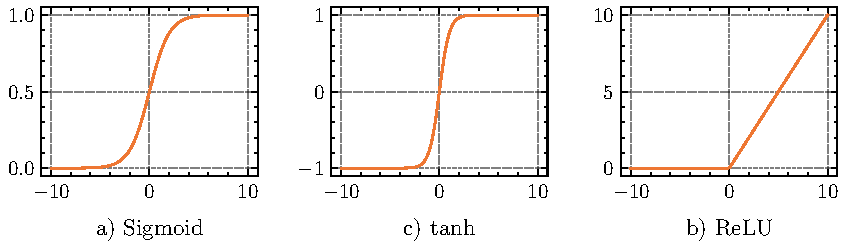
\includegraphics{activations.pdf}
	\caption[Drei weitverbreitete Aktivierungsfunktionen.]{Drei weitverbreitete Aktivierungsfunktionen. \captiona Die Sigmoid-Funktion \captionb der Tangens Hyperbolicus und \captionc die Rectified Linear Unit. Eigene Darstellung (angelehnt an \textcite[4]{Charte.2018})}
	\label{fig:activations}
\end{figure}
Dabei ist in \captiona die (logistische) Sigmoid-Funktion
\begin{equation}
	\label{eq:Sigmoid}
	\operatorname{sigmoid}(x) = \frac{1}{1 + \exp (-x)} \, ,
\end{equation}
in \captionb der \textit{Tangens Hyperbolicus}
\begin{equation}
	\label{eq:tanh}
	\operatorname{tanh}(x) = \frac{\exp(x) - \exp(-x)}{\exp(x) + \exp(-x)}
\end{equation}
und in \captionc die \textit{Rectified Linear Unit}
\begin{equation}
	\label{eq:ReLU}
	\operatorname{ReLU}(x) = \max\{0, x\} \, ,
\end{equation}
abgebildet \parencites[191 -- 195]{Goodfellow.2016}[4]{Charte.2018}. Hierbei bezeichnet $\exp(\, \cdot \,)$ die
Exponentialfunktion. Obwohl ReLU (\eqref{eq:ReLU}) die mittlerweile für neuronale Netze
standardmäßig empfohlene Aktivierungsfunktion ist \parencite[195]{Goodfellow.2016}, wird für Autoencoder die Sigmoid-Funktion (\eqref{eq:Sigmoid})
empfohlen. Dies liegt daran, dass die \textit{Rectified Linear Units} alle negativen Inputs auf
Null projiziert und damit die Rekonstruktion erschweren könnte \parencite[4]{Charte.2018}. Ein möglicher Nachteil der Sigmoid-Funktion ist allerdings der Wertebereich
$[0, 1]$, was eine Rekonstruktion ebenfalls behindern könnte.
\subsection{Contractive Autoencoder}
\label{ch:MethodenDerDimRed:ML:CAE}
\nomenclature[Z]{CAE}{Contractive Autoencoder}

Der Contractive Autoencoder \parencite{Rifai.2011a} stellt eine Variante des eben vorgestellten klassischen Autoencoders
(\subsecref{ch:MethodenDerDimRed:ML:AE}) dar. Ähnlich wie der Sparse Autoencoder wird die
Zielfunktion des Autoencoders lediglich um einen zusätzlichen Regularisierungsterm erweitert.
Dieser zusätzliche Term in der Zielfunktion führt zu einer kontrahierenden Eigenschaft: Ähnliche
Punkte werden auf eine kleinere Nachbarschaft auf der Mannigfaltigkeit abgebildet. Dies gilt aber
nur \textit{lokal}, das heißt unähnliche Punkte können immer noch weit weg auf der Mannigfaltigkeit
liegen \parencite[521]{Goodfellow.2016}. Im Folgenden wird in einem ersten Schritt die Grundidee des
Contractive Autoencoders erläutert und im zweiten Schritt die konkrete Berechnung des
Regularisierungsterms für einen dreischichtigen Autoencoder vorgestellt.

\subsubsection{Grundidee}
\label{ch:MethodenDerDimRed:CAE:Grundidee}

Die Idee ist es, die \textit{Sensitivität} des Autoencoders für den Input zu bestrafen, um damit
eine robustere latente Repräsentation zu erhalten. Das bedeutet, dass bei kleinen Änderungen des
Inputs $\vect{x}$ die Kodierung $f(\vect{x})$ ebenfalls nur minimal geändert werden soll. Dies
entspricht einer kleinen ersten Ableitung und kann über die (quadrierte) Frobeniusnorm der
Jacobi-Matrix $\mat{J}$ des Encoders $f$ erzielt werden \parencites[2]{Rifai.2011a}[521]{Goodfellow.2016}. Der Regularisierungsterm lautet damit
\begin{equation}
	\label{eq:CAE-Regularisierung}
	\Omega(\vect{y}) = \norm[\big]{\mat{J}_f(\vect{x})}_F^2 =  \norm[\Big]{ \frac{\partial f(\vect{x})}{\partial \vect{x}} }^2_F \, ,
\end{equation}
was der Summe über die quadrierten Einträge der Jacobi-Matrix entspricht. Wird angenommen, dass die Daten auf einer $d$-dimensionalen Mannigfaltigkeit liegen, so kann der Regularisierungsterm wie folgt geometrisch interpretiert werden. Einerseits sorgt der Regularisierungsterm dafür, dass der Autoencoder die Kodierung bei einer kleinen Änderung des Inputs nur wenig ändert, d.h. $f(\vect{x})$ soll möglichst konstant sein. Andererseits muss der Autoencoder auch den Rekonstruktionsfehler minimieren, sodass nicht alle Richtungen bei einer Änderung kontrahiert werden dürfen. Diese zwei entgegengesetzten Kräfte kann der Autoencoder gleichzeitig am besten balancieren, wenn die Richtungen parallel zur Mannigfaltigkeit für die stärkste Änderung in der Kodierung verantwortlich sind. In diesen \enquote{lokal relevanten} Richtungen wirkt der Contractive Autoencoder also weniger kontrahierend und die Richtungen, die orthogonal zur Mannigfaltigkeit liegen, werden am stärksten kontrahiert \parencites[1]{Rifai.2011a}[649 -- 650]{Rifai.2011b}.

Der Regularisierungsterm ist für einen dreischichtigen Autoencoder effizient zu berechnen, nicht
aber für einen tiefen Autoencoder. Dies stellt ein praktisches Problem dar, welches allerdings über
ein schichtenweises Vortrainieren teilweise umgangen werden werden kann \parencite[vgl.][522]{Goodfellow.2016}.

\subsubsection{Berechnung des Regularisierungsterms}
\label{ch:MethodenDerDimRed:ML:CAE:BerechnungRegTerm}
Im Folgenden wird die konkrete Berechnung des Regularisierungsterms (\eqref{eq:CAE-Regularisierung}) für einen dreischichtigen Autoencoder aufgezeigt. Wie eben erwähnt, ist die Berechnung in diesem Fall effizient möglich. Bei der mathematischen Formulierung der Autoencoder wurde bereits in \eqref{eq:dreischichtigerAE} die explizite Form des Encoders und Decoders eingeführt. Nimmt man nun an, dass die Gewichte verbunden sind, d.h. $\mat{W}_2 = \tr{\mat{W}_1}$ und wird für die Aktivierungsfunkion $s$ die Sigmoid-Funktion (\eqref{eq:Sigmoid})
verwendet, so kann die Frobeniusnorm der Jacobi-Matrix am Punkt $\vect{x}$ mittels
\begin{equation}
	\label{eq:CAE-loss-simple}
	\norm[\big]{\mat{J}_f(\vect{x})}_F^2 = \sum_{i = 1}^d \left( y^{(i)} \left( 1 - y^{(i)} \right) \right)^2 \sum_{j = 1}^D \big(\mat{W}_1^2\big)_{ij}
\end{equation}
effizient berechnet werden \parencite[4]{Rifai.2011a}. Für einen Autoencoder mit mehr als einer versteckten Schicht wird die
Berechnung teuer, was das Trainieren eines tiefen Contractive Autoencoders ohne Approximationen wie
beispielsweise das von \textcite{Bengio.2006} erläuterte gierige schichtenweise Vortrainieren
(engl. \textit{greedy layer-wise pretraining}) unpraktikabel macht. Bei diesem Vorgehen wird ein
tiefer Autoencoder schichtenweise durch untiefe Autoencoder (drei Schichten) vortrainiert und im
letzten Schritt erfolgt eine Feinabstimmung des kompletten Netzwerks \parencite[522]{Goodfellow.2016}. Dieses Vorgehen kann analog auch für klassische Autoencoder verwendet
werden, um eine gute Initialisierung der Gewichte zu erreichen und damit suboptimale lokale Minima
der Zielfunktion zu umgehen \parencite[509]{Goodfellow.2016}.